\documentclass[conference]{IEEEtran}
\IEEEoverridecommandlockouts
% The preceding line is only needed to identify funding in the first footnote. If that is unneeded, please comment it out.
\usepackage{cite}
\usepackage{amsmath,amssymb,amsfonts}
\usepackage{algorithmic}
\usepackage{graphicx}
\usepackage{textcomp}
\usepackage{xcolor}
\def\BibTeX{{\rm B\kern-.05em{\sc i\kern-.025em b}\kern-.08em
    T\kern-.1667em\lower.7ex\hbox{E}\kern-.125emX}}
\begin{document}

\title{Title of your final project of DS Proseminar}

\author{\IEEEauthorblockN{1\textsuperscript{st} Given Name Surname}
\and
\IEEEauthorblockN{2\textsuperscript{nd} Given Name Surname}
\and
\IEEEauthorblockN{3\textsuperscript{rd} Given Name Surname}
\and
\IEEEauthorblockN{4\textsuperscript{th} Given Name Surname}
}

\maketitle

\section{Introduction}
Shortly summarize the surveillance system problem.  

\section{System architecture}
Describe your system in detail, including a figure for your architectural diagram (IoT, Edge, Cloud layers, components developed and services used).

\begin{figure}[h!]
    \centering
    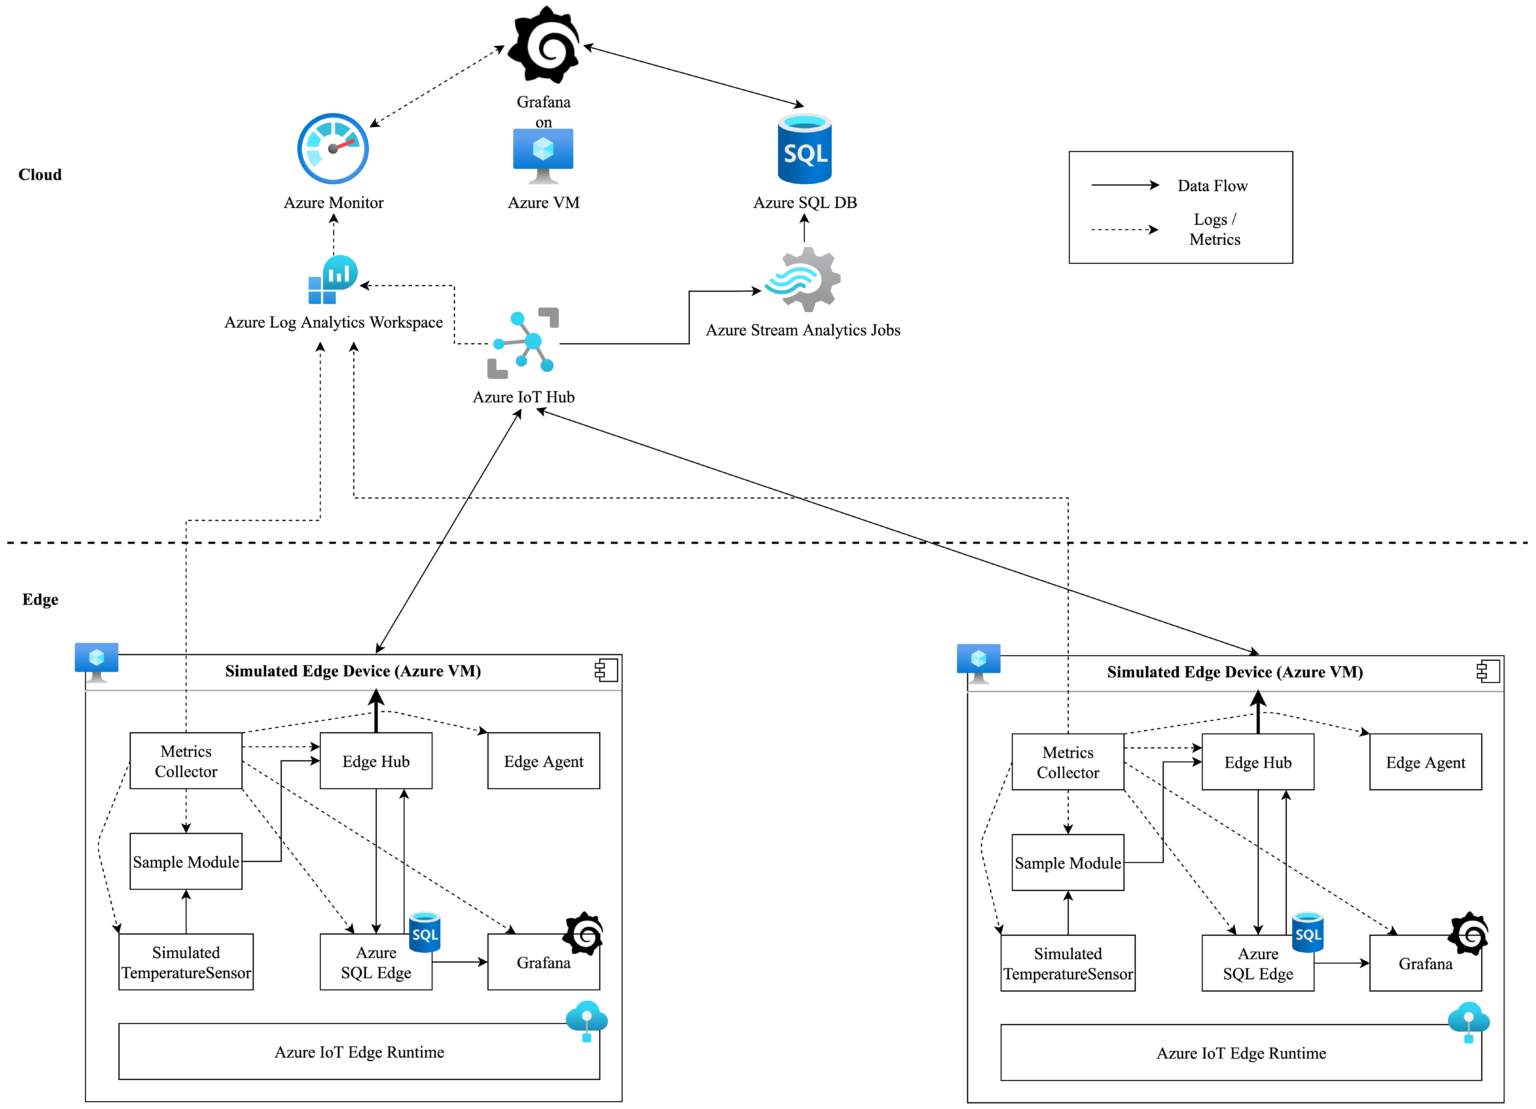
\includegraphics[width=1\linewidth]{image.png}
    \caption{Example of your architectural diagram.}
    \label{fig:enter-label}
\end{figure}

\section{Implementation details}
Provide details about the frameworks and resources used. Justify your decisions carefully.

\section{Evaluation}
Evaluation of the response time and scalability (number of devices and traffic) to prove the correctness of your implementation. The more detailed the better. 

\end{document}
